\newpage

\section{Pengujian dan analisis}
% bab 4 akan menjelaskan hasil train dari model clustering k means yang telah dibuat
Pada bab ini, akan dijelaskan mengenai hasil pengujian dan analisis dari model clustering yang menggunakan algoritma K-Means. Selain itu, akan dipaparkan juga mengenai skenario pengujian yang dilakukan untuk mengevaluasi performa sistem dalam mengelompokkan data pelanggan berdasarkan fitur-fitur yang relevan. Pengujian ini bertujuan untuk memastikan bahwa model K-Means yang dirancang dapat mengidentifikasi pola dalam data dan memberikan hasil yang akurat dalam segmentasi pelanggan.

\subsection{Pengujian Sistem}

Pengujian sistem dilakukan dengan menggunakan dataset yang telah diolah sebelumnya. Data tersebut akan digunakan untuk melatih model clustering K-Means yang diharapkan dapat menghasilkan cluster yang merepresentasikan segmen pelanggan berdasarkan fitur fitur yang dipilih pada bab sebelumnya. Adapun skenario pengujian yang dilakukan adalah sebagai berikut:

\begin{enumerate}
    \item \texttt{Pengujian KMeans} : Data yang telah diolah sebelumnya akan digunakan dalam pelatihan KMeans untuk mendapatkan model clustering yang optimal.
    \item \texttt{Evaluasi Hasil Clustering} : Setelah model KMeans dilatih, hasil clustering akan dievaluasi untuk menentukan seberapa baik model tersebut dalam mengelompokkan data pelanggan.
\end{enumerate}

\subsection{Pengujian KMeans}

Pengujian KMeans dilakukan dengan menggunakan data yang telah dipersiapkan sebelumnya. Data tersebut terdiri dari fitur-fitur yang relevan untuk segmentasi pelanggan, seperti \texttt{SUM\_YR\_1}, \texttt{LAST\_TO\_END}, dan \texttt{AVG\_INTERVAL}. Model KMeans akan dilatih dengan data ini untuk mengidentifikasi pola dan mengelompokkan pelanggan ke dalam cluster yang sesuai.

\subsubsection{Hasil Pengujian KMeans dengan Elbow Method}
Sebelum kita masuk ke hasil clustering, kita perlu menentukan jumlah cluster yang optimal. Salah satu metode yang umum digunakan untuk menentukan jumlah cluster adalah Elbow Method. Metode ini melibatkan perhitungan inertia (dalam hal ini, jarak kuadrat dari titik data ke pusat cluster) untuk berbagai jumlah cluster dan kemudian memplot hasilnya. Gambar \ref{fig:elbow_method} menunjukkan plot Elbow Method yang digunakan untuk menentukan jumlah cluster yang optimal.

\begin{figure}[H]
    \centering
    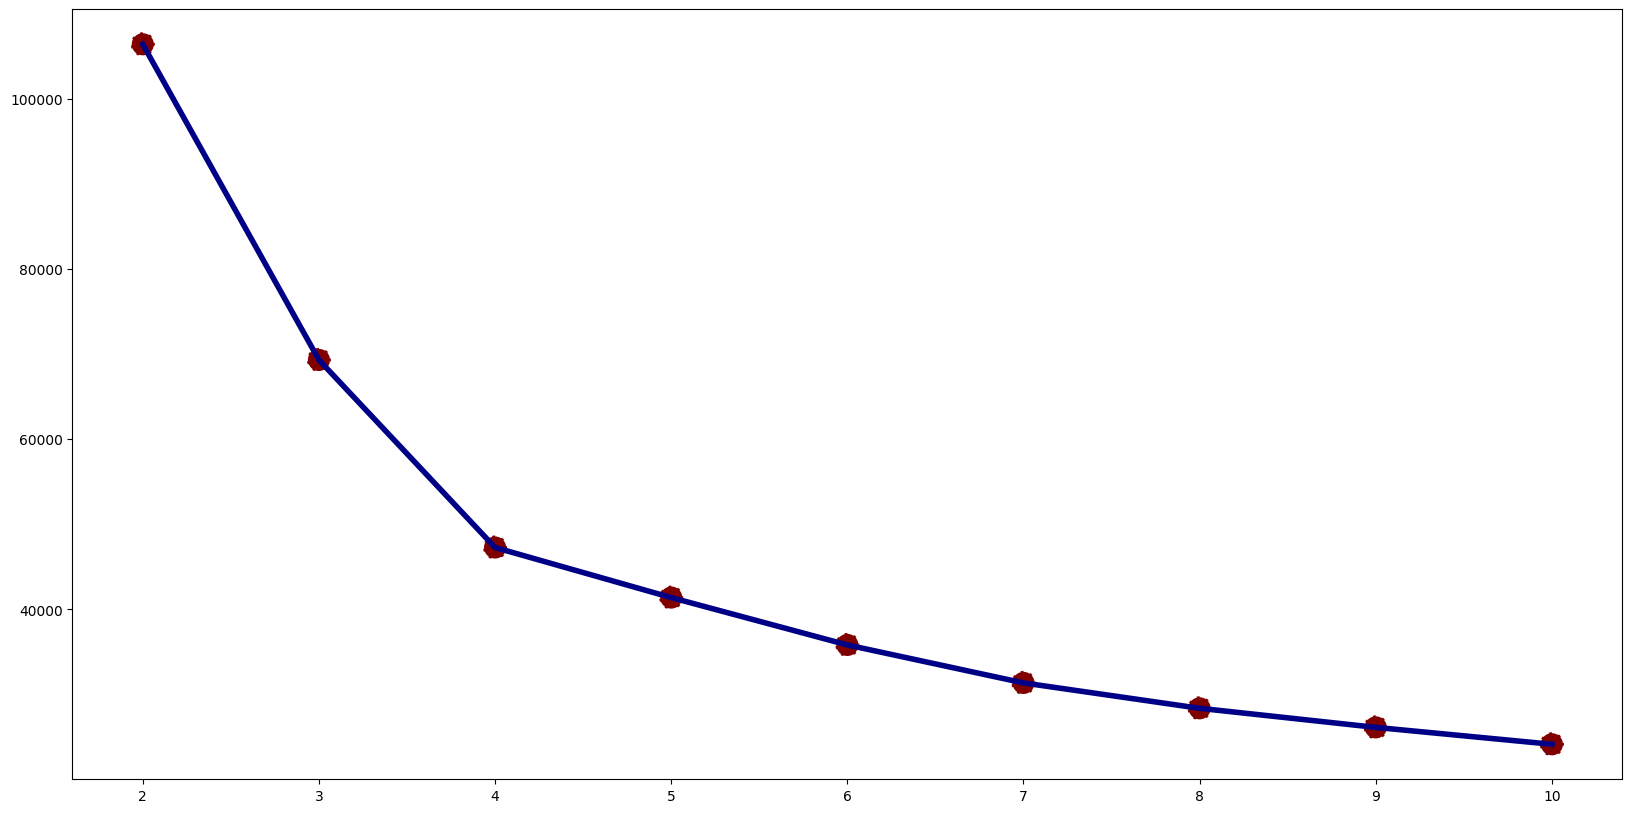
\includegraphics[width=0.5\textwidth]{gambar/ElbowMethod.png}
    \caption{Plot Elbow Method untuk menentukan jumlah cluster optimal}
    \label{fig:elbow_method}
\end{figure}

Didapatkan jumlah cluster yang optimal adalah 4, karena pada titik tersebut terjadi penurunan inertia yang signifikan sehingga cluster tersebut akan digunakan untuk visualisasi hasil clustering KMeans selanjutnya.

\subsubsection{Hasil Clustering KMeans}
Setelah menentukan jumlah cluster yang optimal, model KMeans dilatih dengan data yang telah disiapkan. Hasil clustering menunjukkan bahwa pelanggan dikelompokkan ke dalam 4 cluster yang berbeda. Gambar \ref{fig:kmeans_clusters} menunjukkan hasil clustering 3D Plot untuk KMeans yang telah dilakukan.

\begin{figure}[H]
    \centering
    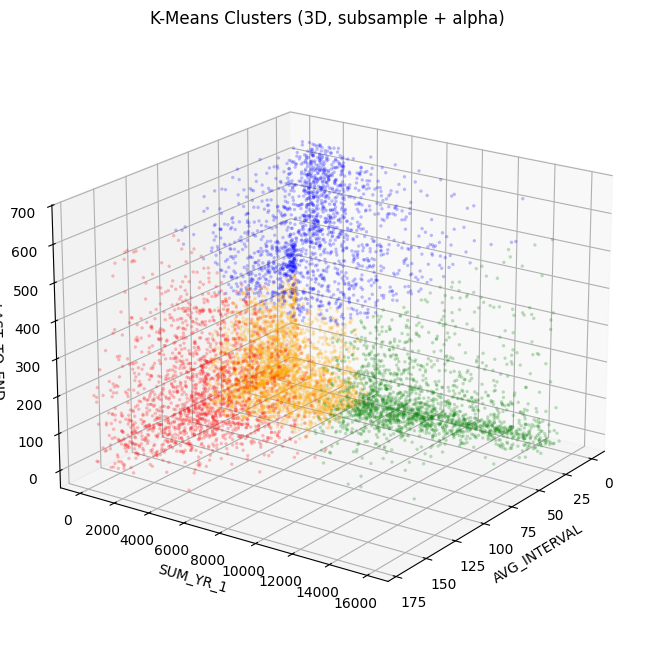
\includegraphics[width=0.65\textwidth]{gambar/hasilkmeans2.png}
    \caption{Hasil Clustering KMeans 3D Plot}
    \label{fig:kmeans_clusters}
\end{figure}

Dari plot 3D di atas, kita dapat melihat bahwa pelanggan dikelompokkan ke dalam 4 cluster yang berbeda berdasarkan fitur-fitur yang telah dipilih. Setiap titik mewakili pelanggan, dan warna yang berbeda menunjukkan cluster yang berbeda. Hal ini menunjukkan bahwa model KMeans berhasil mengidentifikasi pola dalam data dan mengelompokkan pelanggan dengan cara yang bermakna.

Adapun warna yang digunakan untuk setiap segmen adalah sebagai berikut:
\begin{itemize}
    \item Segmen VIP : Hijau
    \item Segmen Customer Active Frequent Low Spender : Kuning
    \item Segmen Lapsed Frequent Low Spender : Biru
    \item Segmen Occasional Low Value : Merah
\end{itemize}

Dari hasil tersebut kita telah mendapatkan 4 segmen pelanggan yang berbeda, yang masing-masing memiliki karakteristik dan perilaku yang unik. Hal ini memungkinkan perusahaan untuk merancang strategi pemasaran yang lebih efektif dan terfokus pada setiap segmen pelanggan.

Selain menggunakan 3D plot kita juga akan menggunakan PCA untuk memvisualisasikan hasil clustering KMeans. Gambar \ref{fig:pca_kmeans} menunjukkan hasil PCA yang digunakan untuk mengurangi dimensi data dan memvisualisasikan cluster dalam 2D.

\begin{figure}[H]
    \centering
    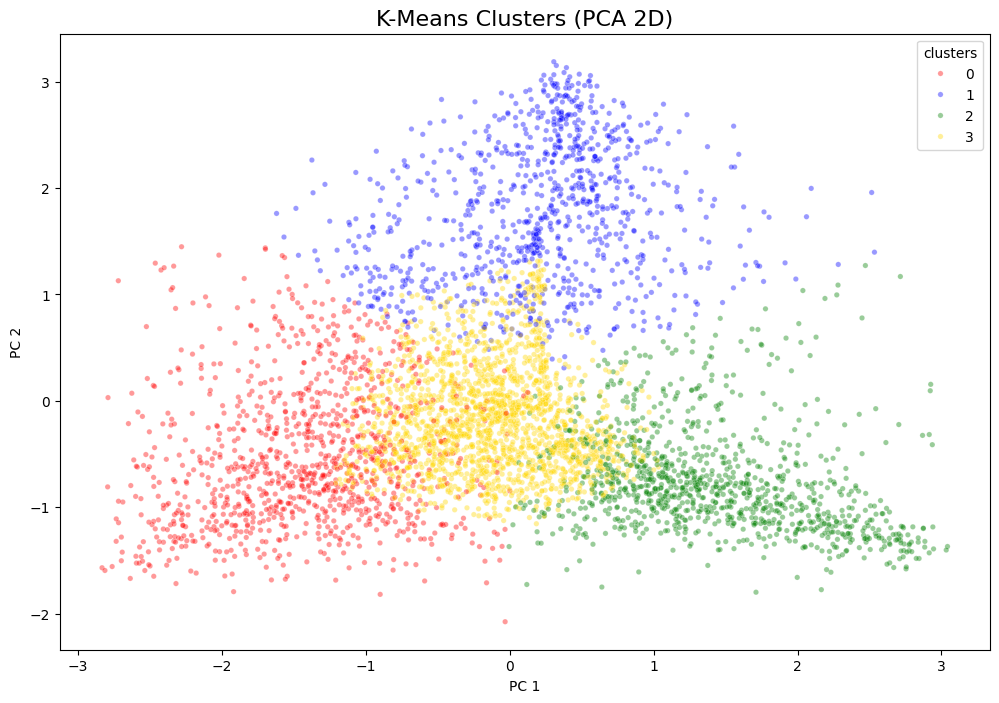
\includegraphics[width=0.65\textwidth]{gambar/PCA.png}
    \caption{Hasil PCA Clustering KMeans 2D Plot}
    \label{fig:pca_kmeans}
\end{figure}

Dari plot PCA di atas, kita dapat melihat bahwa pelanggan dikelompokkan ke dalam 4 cluster yang berbeda dengan jelas. Setiap titik mewakili pelanggan, dan warna yang berbeda menunjukkan cluster yang berbeda. Hal ini menunjukkan bahwa model KMeans berhasil mengidentifikasi pola dalam data dan mengelompokkan pelanggan dengan cara yang bermakna.

Selain dari plot didapatkan juga ukuran pemusatan dari hasil Clustering KMeans yang telah dilakukan. Tabel \ref{tab:cluster_summary} menunjukkan pusat dari setiap cluster yang dihasilkan oleh model KMeans.

% SUM_YR_1	LAST_TO_END	AVG_INTERVAL
% clusters	mean	    median	mean	median	mean	median					
% 0	        2027.909230	1709.0	149.954424	123.0	111.947414	107.000000
% 1	        3189.024061	2639.5	462.502805	463.0	31.555278	27.775000
% 2	        9795.947353	9294.0	79.781578	42.0	35.590739	32.547727
% 3	        2035.480580	1700.0	89.106335	69.0	42.410628	43.600000

\begin{table}[H]
    \centering
    \caption{Statistik Rata-rata dan Median per Cluster}
    \label{tab:cluster_summary}
    \begin{tabular}{|c|c|c|c|c|c|c|}
        \hline
        \multirow{2}{*}{Cluster} & \multicolumn{2}{c|}{SUM\_YR\_1} & \multicolumn{2}{c|}{LAST\_TO\_END} & \multicolumn{2}{c|}{AVG\_INTERVAL} \\
        \cline{2-7}
         & Mean & Median & Mean & Median & Mean & Median \\
        \hline
        0 & 2027.91 & 1709.0 & 149.95 & 123.0 & 111.95 & 107.0 \\
        1 & 3189.02 & 2639.5 & 462.50 & 463.0 & 31.56  & 27.78 \\
        2 & 9795.95 & 9294.0 & 79.78  & 42.0  & 35.59  & 32.55 \\
        3 & 2035.48 & 1700.0 & 89.11  & 69.0  & 42.41  & 43.60 \\
        \hline
    \end{tabular}
\end{table}

Tabel di atas menunjukkan rata-rata dan median dari setiap fitur untuk masing-masing cluster. Dari tabel tersebut, kita dapat melihat perbedaan yang signifikan antara cluster yang satu dengan yang lainnya. Hal ini menunjukkan bahwa model KMeans berhasil mengidentifikasi pola dalam data dan mengelompokkan pelanggan dengan cara yang bermakna.

\subsection{Interpretasi Hasil Clustering}
% \begin{enumerate}
%     \item Recency Rendah, Frequency Rendah, Monetary Tinggi merupakan Customer VIP.
%     \item Recency Rendah, Frequency Rendah, Monetary Rendah merupakan Customer Active Frequent Low Spender.
%     \item Recency Tinggi, Frequency Rendah, Monetary Rendah merupakan Lapsed Frequent Low Spender.
%     \item Recency Rendah, Frequency Tinggi, Monetary Rendah merupakan Occasional Low Value.
% \end{enumerate}
Interpretasi hasil clustering KMeans memberikan wawasan yang berharga tentang segmen pelanggan yang berbeda. Berdasarkan hasil clustering, kita dapat mengidentifikasi empat segmen pelanggan yang berbeda, masing-masing dengan karakteristik dan perilaku yang unik. Namun sebelum itu Tabel \ref{tab:cluster_summary} di atas memberikan tabel makna dari masing masing RFM:

\begin{table}[H]
    \centering
    \caption{Makna dari masing-masing RFM}
    \label{tab:rfm_meaning}
    \begin{tabular}{|c|c|}
        \hline
        RFM & Makna \\
        \hline
        Recency Rendah, Frequency Rendah, Monetary Tinggi & Customer VIP \\
        Recency Rendah, Frequency Rendah, Monetary Rendah & Customer Active Frequent Low Spender \\
        Recency Tinggi, Frequency Rendah, Monetary Rendah & Lapsed Frequent Low Spender \\
        Recency Rendah, Frequency Tinggi, Monetary Rendah & Occasional Low Value \\
        \hline
    \end{tabular}
\end{table}

Di mana :
\begin{itemize}
    \item Semakin rendah Recency berarti pelanggan tersebut semakin baru melakukan transaksi, berdasarkan makna dari fitur LAST\_TO\_END.
    \item Semakin rendah Frequency berarti pelanggan tersebut semakin sering melakukan transaksi, berdasarkan makna dari fitur AVG\_INTERVAL.
    \item Semakin tinggi Monetary berarti pelanggan tersebut semakin mahal transaksinya, berdasarkan makna dari fitur SUM\_YR\_1.
\end{itemize}

Sehingga bisa kita lakukan Interpretasi dari 4 cluster yang didapatkan berdasarkan warna yang ada pada hasil clustering KMeans:


\begin{enumerate}
    \item \textbf{Segmen VIP (Hijau)}: Pelanggan dengan Recency rendah, Frequency rendah, dan Monetary tinggi. Mereka adalah pelanggan yang jarang bertransaksi tetapi ketika bertransaksi, mereka mengeluarkan uang dalam jumlah besar. Ini menunjukkan bahwa mereka adalah pelanggan yang sangat berharga bagi perusahaan.
    \item \textbf{Segmen Customer Active Frequent Low Spender (Kuning)}: Pelanggan dengan Recency rendah, Frequency rendah, dan Monetary rendah. Mereka adalah pelanggan yang sering bertransaksi tetapi dengan nilai transaksi yang rendah. Ini menunjukkan bahwa mereka adalah pelanggan yang aktif tetapi tidak mengeluarkan banyak uang.
    \item \textbf{Segmen Lapsed Frequent Low Spender (Biru)}: Pelanggan dengan Recency tinggi, Frequency rendah, dan Monetary rendah. Mereka adalah pelanggan yang jarang bertransaksi dan ketika bertransaksi, mereka mengeluarkan uang dalam jumlah kecil. Ini menunjukkan bahwa mereka mungkin telah kehilangan minat pada produk atau layanan perusahaan.
    \item \textbf{Segmen Occasional Low Value (Merah)}: Pelanggan dengan Recency rendah, Frequency tinggi, dan Monetary rendah. Mereka adalah pelanggan yang sering bertransaksi tetapi dengan nilai transaksi yang sangat rendah. Ini menunjukkan bahwa mereka mungkin hanya membeli produk atau layanan dengan harga murah.
\end{enumerate}

Dengan memahami karakteristik masing-masing segmen pelanggan, perusahaan dapat merancang strategi pemasaran yang lebih efektif dan terfokus pada setiap segmen. Misalnya, perusahaan dapat menawarkan promosi khusus kepada pelanggan VIP untuk meningkatkan loyalitas mereka, atau menawarkan diskon kepada pelanggan Lapsed Frequent Low Spender untuk menarik mereka kembali bertransaksi.
